\section{User Interface}
\label{sec:chapter_2_section_2}

La \emph{User Interface} ha un ruolo importante perché tramite essa vengono azionate tutte le funzionalità
implementate dal framework. L'area di lavoro (Figura~\ref{fig:interfaccia}) è suddivisa in tre sottoparti:
\begin{itemize}
  \item toolbar
  \item content-area
  \item sidebar
\end{itemize}

\begin{figure}[htbp] %  figure placement: here, top, bottom, or page
   \centering
   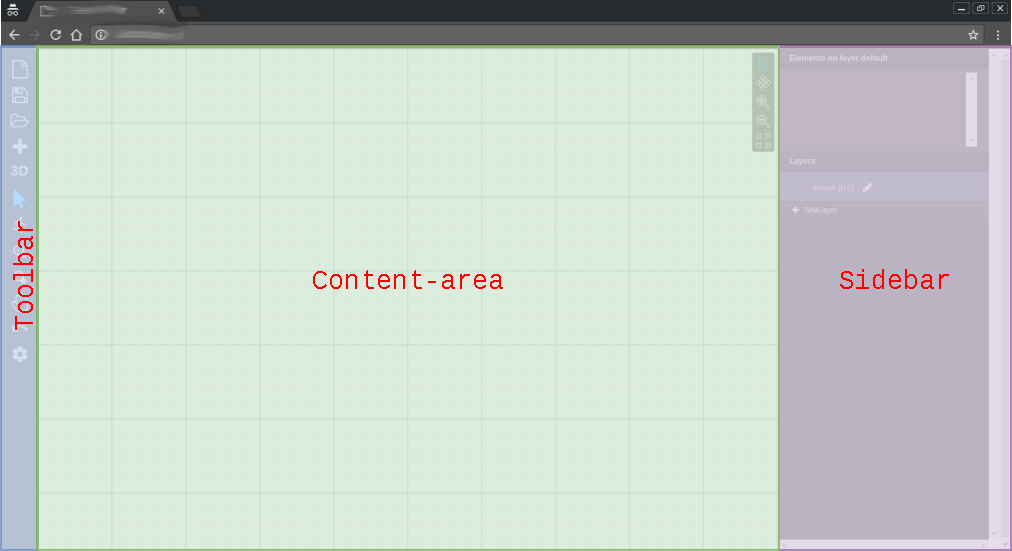
\includegraphics[width=1\linewidth]{images/mock-interfaccia}
   \caption{Schermata interfaccia utente}
   \label{fig:interfaccia}
\end{figure}

Dalla \emph{toolbar} l'utente pu\`o accedere alle funzionalit\`a relative a: ciclo di vita del progetto (new, save, load);
switching modalità vista/interazione (2D, 3D); cambio di modalità di interazione (selecting, pan, zoom).
\newpage
La \emph{content-area} \`e l'area nella quale l'utente pu\`o interagire con il modello attuale. Nella modalit\`a 2D
il modello \`e visualizzato come una proiezione 2D dall'alto e l'interazione consiste nell'inserimento, selezione e modifica
dell'elemento (in accordo con le specifiche interattive del building element). Nella modalità 3D un modello 3D pu\`o essere
ispezionato e navigato attraverso due modalità differenti: in prima persona usando il mouse e la tastiera ponendo la vista
ad altezza uomo, o dall'alto cambiando la posizione della telecamera con il solo mouse. Anche in modalità 3D è possibile
selezionare e modificare le proprietà degli oggetti.\\
\indent
La \emph{sidebar} visualizza le propriet\`a dell'elemento correntemente selezionato. Nel pannello delle propriet\`a \`e possibile
vedere la descrizione dell'elemento, aggiungere/rimuovere metadati, e modificare qualsiasi propriet\`a.
Quest'ultima modalità di interazione consente al utente di associare annotazioni semantiche su ogni parte del modello.
\newpage

\subsection{Viewer 2D}
Il \emph{2D-viewer} invoca la funzione \emph{2Dgf} dei \emph{building elements} aggiunti al modello e
genera in output il modello renderizzato usando gli elementi SVG.
Per far fronte ai frequenti aggiornamenti provenienti dall'interazione con il disegno da parte dell'utente,
sfrutta una \emph{Virtual DOM}~\cite{vdom}, che permette di aggiornare solo la parte modificata evitando così
il completo rendering della scena. Per eseguire le operazioni di pan e zoom, tipicamente necessaria in questo
tipo di strumento, è stato sviluppato un componente ad-hoc di React denominato \emph{ReactSVGPanZoom}~\cite{panzoom}.\\


\begin{figure}[htbp] %  figure placement: here, top, bottom, or page
   \centering
   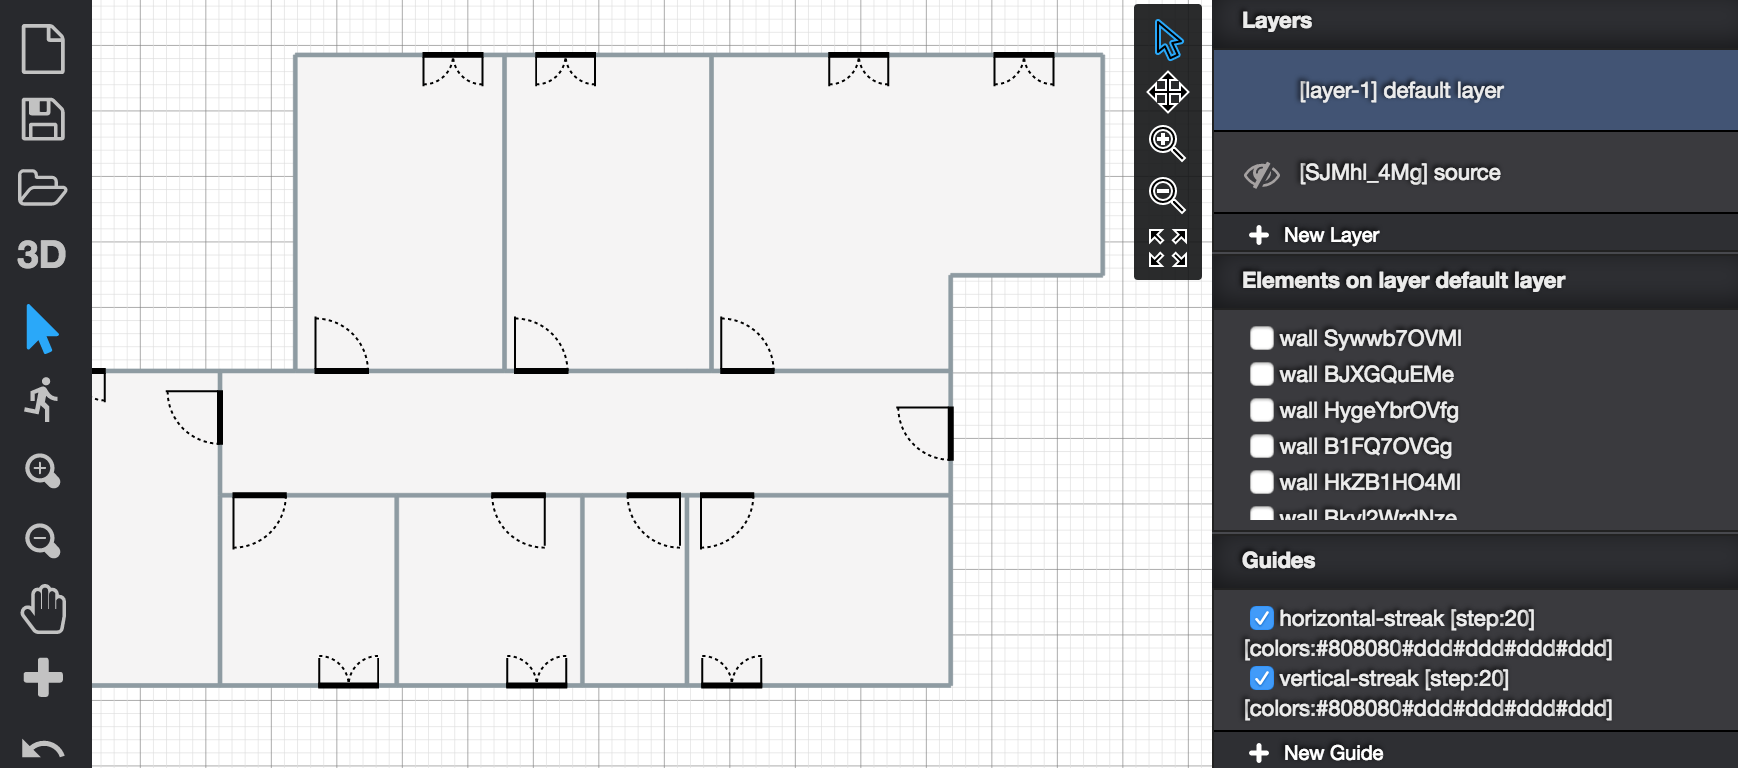
\includegraphics[width=1\linewidth]{images/2d}
   \caption{Schermata viewer 2D}
   \label{fig:view2D}
\end{figure}
\newpage


\subsection{Viewer 3D}
Il \emph{3D-viewer} invoca la funzione \emph{3Dgf} dei \emph{building elements} e aggiunge al modello una vista 3D usando
le primitive WebGL\emph{Three.js}~\cite{threejs-site}.
In particolare durante l'interazione con la scena si dispone delle seguenti \textit{operazioni} sui \emph{Plugin}:
\begin{itemize}
  \item \emph{add};
  \item \emph{replace};
  \item \emph{remove};
\end{itemize}
Per eseguire l'update è stato implementato un \emph{diff} e \emph{patch} di
sistema, definite nel Jsonpatch~\cite{rfc6902}: gli oggetti Three.js sono associati con elementi costruttivi all'interno
dello stato dell'applicazione, in modo che ogni volta che l'utente attiva un'azione che si traduce in una modifica dello stato,
l'applicazione calcola la differenza tra il vecchio stato e quello nuovo e aggiorna solo l'oggetto interessato.\\


\begin{figure}[htbp] %  figure placement: here, top, bottom, or page
   \centering
   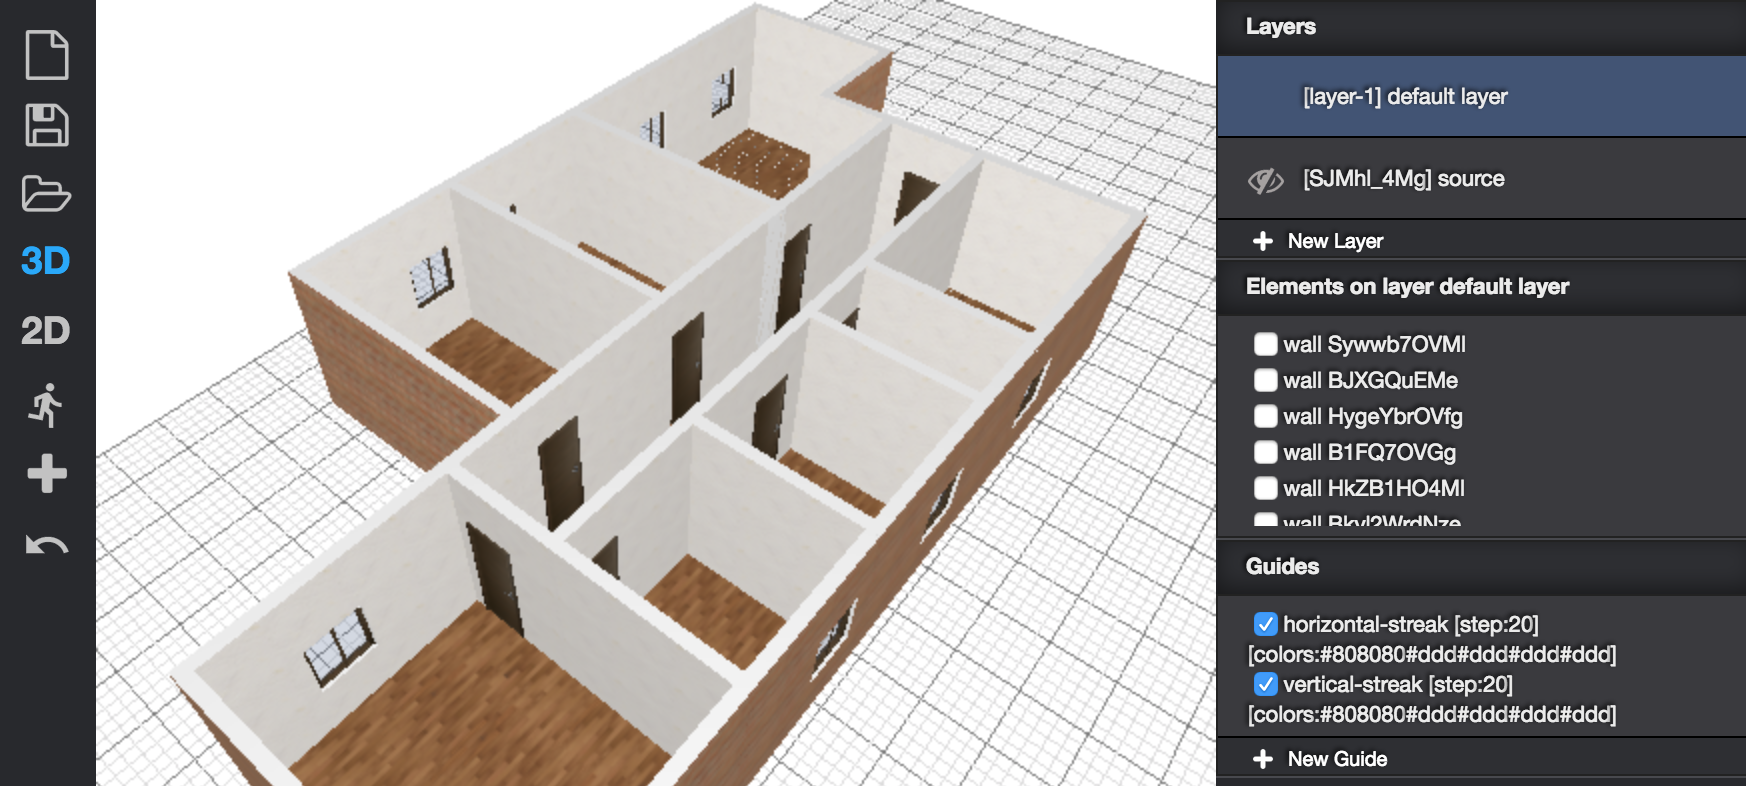
\includegraphics[width=1\linewidth]{images/3d}
   \caption{Schermata viewer 3D }
   \label{fig:viewer3D}
\end{figure}
\newpage

\subsection{Plugin Catalog}
\label{sec:chapter_2_section_2_sub_3}

\noindent
 Il \emph{Plugin Catalog} \`e l'elemento centrale che fornisce all'utente un sistema con un ricco catalogo di \emph{Plugin},
 in cui ogni elemento presente \`e definito da un nome, una descrizione ed una
 immagine di anteprima del modello 3D (Figura~\ref{fig:catalogo} (a)). Quando l'utente \`e al suo interno
 sceglie il \emph{Plugin} che vuole inserire con un click.
 Dopo la selezione di un elemento del catalogo, il framework cambierà il suo stato portandosi nella modalit\`a 2D,
 dove l'utente potrà decidere il posizionamento del \emph{Plugin} all'interno della scena.
 La selezione di un \emph{Plugin} evidenzia l'oggetto con un colore diverso da quello di default ed una circonferenza sulla quale è presente un pallino
 che consente la rotazione dell'oggetto (Figura~\ref{fig:catalogo} (b)).

\begin{figure}[htbp]
\begin{center}
\begin{tabular}{c @{\hspace{1em}} c}
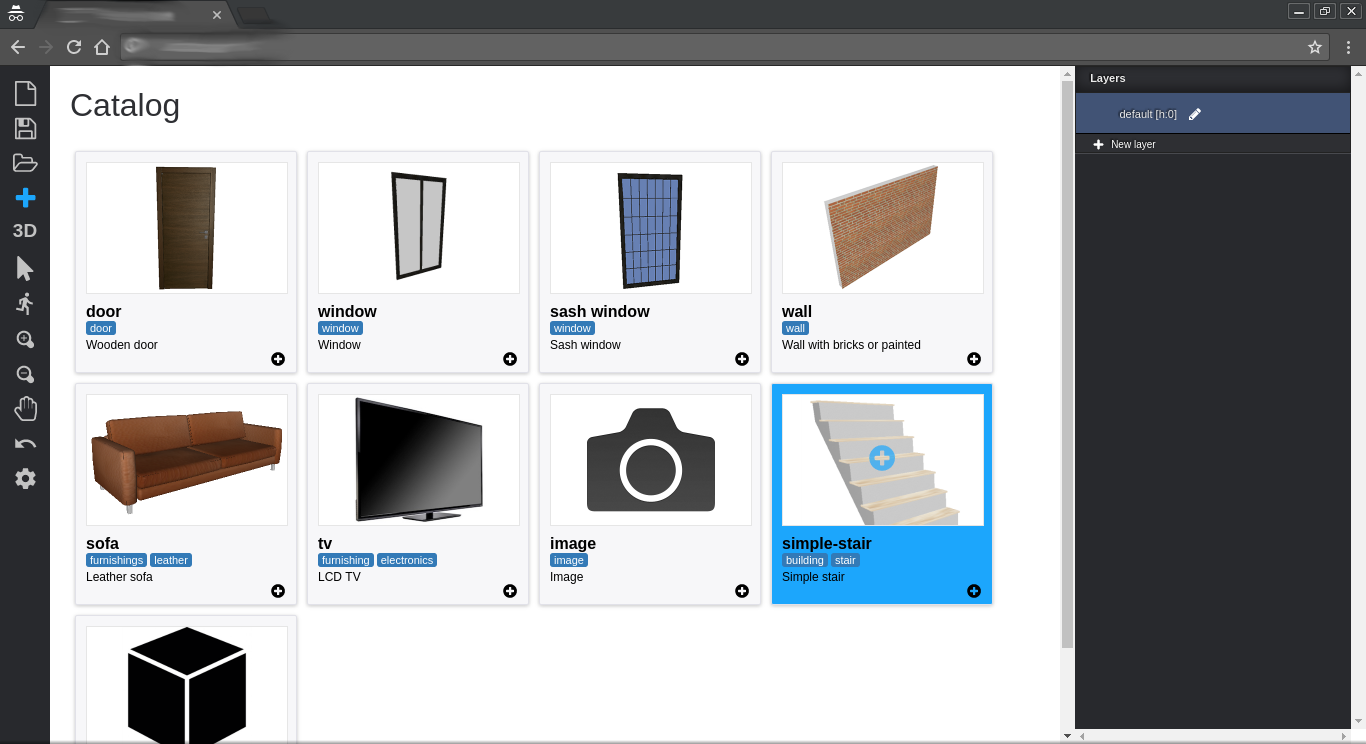
\includegraphics[width=.6\linewidth]{images/figcatalog} \\
  (a) \\
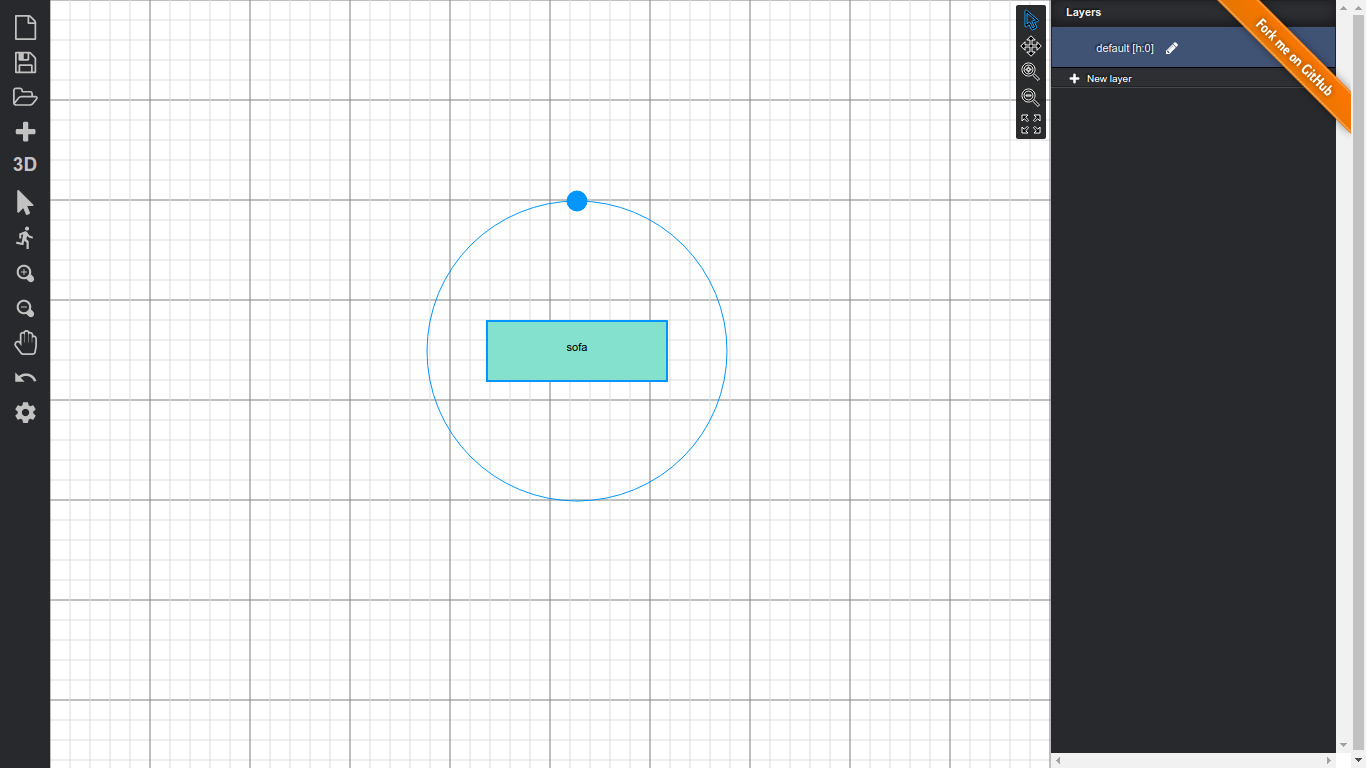
\includegraphics[width=.6\linewidth]{images/positioning} \\
  (b) \\
\end{tabular}
\end{center}
\caption{Dettaglio Plugin: (a) Vista dei plugin nel catalogo, (b) inserimento oggetto dopo la selezione nel catalogo}\label{fig:catalogo}
\end{figure}
\newpage
